\subsection{Komponen \textit{Predictor}}
Komponen \textbf{\textit{Predictor}} terdiri dari 3 buah kelas, yaitu sebagai berikut.
\begin{enumerate}
    \item \textbf{\textit{Predict Component}}
    
    Kelas ini berfungsi untuk menyimpan sebuah model ARIMA untuk sebuah variabel. Kelas ini memanfaatkan kakas pandas, statsmodels dan pmdarima untuk melakukan tanggung jawabnya.

    \item \textbf{\textit{Predict Component Factory}}
    
    Kelas ini berfungsi untuk membuat objek \textbf{\textit{Predict Component}} sebanyak variabel yang ada. 

    \item \textbf{\textit{Predict Component Storage}}
    
    Kelas ini berfungsi sebagai aggregator objek \textbf{\textit{Predict Component}} yang telah dibuat oleh \textbf{\textit{Predict Component Factory}}. Kelas ini juga berfungsi untuk meneruskan sebuah aksi kepada semua objek \textbf{\textit{Predict Component}} yang ada. Contohnya, dengan memanggil \textit{forecast} atau \textit{update data}, maka operasi akan diteruskan ke semua objek \textbf{\textit{Predict Component}}.

\end{enumerate}

\begin{figure}[h]
    \centering
    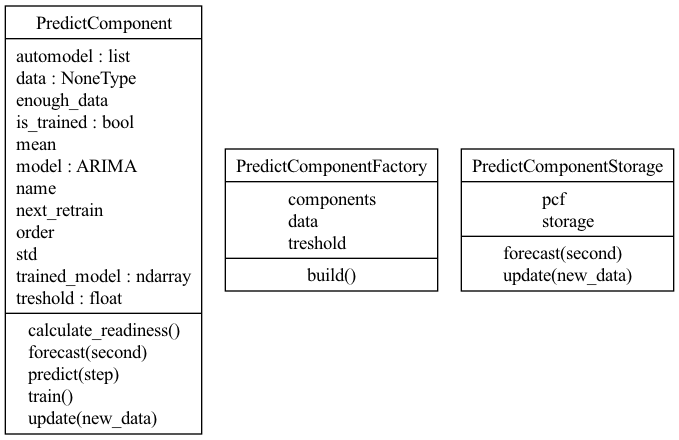
\includegraphics[width=0.8\textwidth]{chapter-4/predictor.png}
    \caption{Spesifikasi Kelas Penyusun Komponen \textit{Predictor}}
    \label{fig:predictor-spek}
\end{figure}

Secara umum, spesifikasi kelas bisa dilihat pada gambar \ref{fig:predictor-spek}. Kelas \textbf{\textit{Predict Component Storage}} akan membutuhkan \textbf{\textit{Predict Component Factory}} untuk membangun semua \textbf{\textit{Predict Component}} untuk setiap variabel yang ada. Setelah itu, terdapat operasi seperti meneruskan penambahan data serta meminta data prediksi ke setiap \textbf{\textit{Predict Component}}. Kelas ini akan digunakan oleh komponen \textbf{\textit{Flexible Control}} untuk lebih lanjutnya.

Selama program berjalan, data akan terus masuk karena \textbf{\textit{Metrics Fetcher}} terus menarik data setiap satuan waktu tertentu, oleh karena itu, komponen akan menyesuaikan model dengan data terbaru atau dengan kata lain melakukan \textit{retraining}. Pendekatan yang dibuat adalah dengan membuat sebuah \textit{offset} yang dapat dikonfigurasi, lihat bagian \ref{sec:komponen-pendukung}. Untuk menentukan waktu melakukan \textit{retraining}, maka akan dilakukan perhitungan dengan persamaan \ref{eq:retrain-time}. $\lambda(x)$ bisa disebut sebagai panjang data historis saat training untuk ke-$x$ kalinya dengan $c$ sebagai sebuah konstanta dan $p$ sebagai sebuah persentase. $c$ dan $p$ dapat diubah oleh pengguna sesuai kebutuhan melalui konfigurasi. Dengan kata lain, untuk melakukan training ke-$x$ kalinya, panjang data historis saat itu harus melebihi atau sama dengan $\lambda(x)$. Sebagai contoh, apabila \textit{training} pertama kali membutuhkan 100 data, dengan $c$ sejumlah $50$ dan $p$ sebesar $0.7$, maka \textit{training} kedua kali akan dilakukan ketika data historis sudah mencapai 120 data yang didapat dari $50+0.7*100$. Sebagai catatan, pada saat \textit{training} pertama kali, maka $\lambda(x)$ akan bernilai $c$, dan fitur prediksi tidak akan berjalan sampai \textit{training} dilakukan.

\begin{equation}
    \label{eq:retrain-time}
    \lambda(x) =
        \left\{
        \begin{array}{cl}
            c + p*\lambda(x-1) & : \ x \geq 1 \\
            0 & : \ x < 1
        \end{array}
        \right.
\end{equation}

Selain dari skema \textit{retraining} yang disebutkan sebelumnya, \textbf{\textit{Predict Component}} juga memiliki proses khusus terhadap data yang masuk dan berdampak ketika mengembalikan angka prediksi. Sebagai contoh kasusnya adalah sebagai berikut.
\begin{enumerate}
    \item Ketika mean dari data historis bernilai nol dan standar deviasi bernilai nol.
    \item Ketika data stasioner, yang berarti mean tidak nol namun standar deviasi bernilai nol.
    \item Kondisi normal, mean tidak nol dan standar deviasi tidak nol.
\end{enumerate}

Hal ini dilakukan untuk menghindari \textit{error} yang terjadi ketika melakukan \textit{training} dengan data yang bernilai nol ataupun yang bersifat statis. Proses khusus ini dapat direpresentasikan dengan persamaan yang dapat dilihat pada persamaan \ref{eq:predict-function}. Pada persamaan tersebut, $y(t)$ adalah hasil prediksi di waktu $t$, $ARIMA(t)$ adalah hasil prediksi dari model ARIMA di waktu $t$, $mean$ adalah nilai rata-rata dari data historis, dan $std$ adalah nilai standar deviasi dari data historis di. Pada persamaan tersebut, $mean$ akan selalu bernilai positif atau nol dikarenakan data yang digunakan adalah data yang bernilai positif seperti \textit{request time}, \textit{process time}, \textit{memory used percent}, \textit{cpu percent} dan \textit{load average}. $mean$ dan $std$ akan selalu diperbaharui setiap kali melakukan \textit{training}.

\begin{equation}
    \label{eq:predict-function}
    y(t) = \left\{
        \begin{array}{cl}
            ARIMA(t) & : \ mean > 0, std > 0 \\
            mean & : \ mean > 0, std = 0 \\
            NaN & : \ mean = 0, std = 0 \\
        \end{array}
    \right.
\end{equation}